\documentclass[12pt,a4paper]{article}
\usepackage[utf8]{inputenc}
\usepackage[spanish,es-tabla]{babel}
\usepackage{geometry}
\usepackage{graphicx}
\usepackage{multirow}
\usepackage{tabularx}
\usepackage{mathptmx}
\usepackage{fancyhdr}
\usepackage{array}
\usepackage[table]{xcolor}
\usepackage{titlesec}
\usepackage{setspace}
\usepackage{microtype}
\usepackage{lastpage}
\usepackage{booktabs}
\usepackage{enumitem}
\usepackage{amsmath}
\usepackage{amsfonts}
\usepackage{amssymb}

\graphicspath{{images/}{../images/}{./}}

\geometry{
    top=4.7cm,
    bottom=2.5cm,
    left=2.5cm,
    right=2.5cm,
    headheight=3.9cm,
    headsep=0.4cm
}

\setstretch{1.15}
\setlength{\parindent}{0pt}
\setlength{\parskip}{0.45em}
\setlength{\tabcolsep}{4pt}

\titleformat{\section}
  {\normalfont\fontsize{12}{14.5}\bfseries}{\thesection.}{0.6em}{\uppercase}
\titlespacing*{\section}
  {0pt}{1.8ex plus 0.4ex minus 0.2ex}{0.6ex plus 0.2ex}

\titleformat{\subsection}
  {\normalfont\fontsize{11.5}{13.5}\bfseries}{\thesubsection.}{0.5em}{}
\titlespacing*{\subsection}
  {0pt}{1.4ex plus 0.3ex minus 0.1ex}{0.4ex plus 0.1ex}

\titleformat{\subsubsection}
  {\normalfont\fontsize{10.5}{12.5}\bfseries\itshape}{\thesubsubsection.}{0.4em}{}
\titlespacing*{\subsubsection}
  {0pt}{1.1ex plus 0.2ex minus 0.1ex}{0.3ex plus 0.1ex}

\newcolumntype{Y}{>{\centering\arraybackslash}X}
\newcolumntype{L}{>{\raggedright\arraybackslash}X}
\newcolumntype{C}{>{\centering\arraybackslash}X}

\definecolor{headerred}{RGB}{180, 0, 0}
\definecolor{darkred}{RGB}{140, 0, 0}
\definecolor{lightgraybg}{RGB}{248, 248, 248}
\definecolor{tableheader}{RGB}{232, 238, 246}

\newcommand{\docCodigo}{TI-SIGE-ENT-S2-001}
\newcommand{\docVersion}{1.0}
\newcommand{\docProceso}{DISEÑO DE SOFTWARE / CASOS DE USO UML}
\newcommand{\docElaboracion}{27/08/2026}
\newcommand{\docRevision}{PENDIENTE DE REVISIÓN}
\newcommand{\docTitulo}{DIAGRAMA GENERAL Y ESPECIFICACIÓN DETALLADA DE CASOS DE USO UML}
\newcommand{\docOrganizacion}{FACULTAD DE INGENIERÍA EN SISTEMAS, ELECTRÓNICA E INDUSTRIAL}
\newcommand{\docSubOrganizacion}{CARRERA DE INGENIERÍA DE SOFTWARE}

\newcommand{\encabezadofrecuente}{%
    \renewcommand{\arraystretch}{1.15}%
    \noindent\makebox[\textwidth][c]{%
    \begin{tabularx}{\textwidth}{|>{\centering\arraybackslash}m{2.8cm}|Y|>{\centering\arraybackslash}m{4.8cm}|}
        \hline
        \multirow{4}{2.8cm}{\centering\raisebox{-1.15cm}{
\includegraphics[width=2.5cm,height=2.0cm,keepaspectratio]{images/logo.png}}}
        & \textbf{\fontsize{9}{11}\selectfont \docOrganizacion} 
        & \textbf{\fontsize{8}{10}\selectfont CÓDIGO:} \fontsize{8}{10}\selectfont \docCodigo \\
        \cline{3-3}
        & \textbf{\fontsize{8.5}{10.5}\selectfont \docSubOrganizacion} 
        & \textbf{\fontsize{8}{10}\selectfont VERSIÓN:} \fontsize{8}{10}\selectfont \docVersion \\
        \cline{2-3}
        & \textbf{\fontsize{8}{10}\selectfont PROCESO:} \fontsize{8}{10}\selectfont \docProceso 
        & \textbf{\fontsize{8}{10}\selectfont ELABORACIÓN:} \fontsize{8}{10}\selectfont \docElaboracion \\
        \cline{2-3}
        & \textbf{\fontsize{8.5}{10.5}\selectfont \docTitulo} 
        & \textbf{\fontsize{8}{10}\selectfont ÚLTIMA REVISIÓN:} \fontsize{8}{10}\selectfont \textbf{\textcolor{darkred}{\docRevision}} \\
        \hline
    \end{tabularx}%
    }%
}

\pagestyle{fancy}
\fancyhf{}
\fancyhead[C]{\encabezadofrecuente}
\fancyfoot[C]{\fontsize{10}{12}\selectfont Página \thepage\ de \pageref{LastPage}}
\renewcommand{\headrulewidth}{0pt}

\begin{document}

\section{Título}
\textbf{Denominación del Entregable:} Modelado General y Especificación Detallada de Casos de Uso del Sistema (EDT 2.1)

\vspace{0.15cm}
\noindent
\textbf{Ficha Técnica de Identificación:}
\begin{itemize}[leftmargin=1.5em, itemsep=1.5pt, topsep=1.5pt]
    \item \textbf{Código Documental:} \docCodigo \quad | \quad \textbf{Versión:} \docVersion
    \item \textbf{Institución:} Universidad Técnica de Ambato (UTA) -- FISEI
    \item \textbf{Carrera:} Ingeniería de Software (Séptimo Semestre "A")
    \item \textbf{Módulo Académico:} Gestión de Proyectos de Software
    \item \textbf{Docente Tutor:} Ing. Paulo Torres
    \item \textbf{Fecha de Elaboración:} \docElaboracion \quad | \quad \textbf{Estado:} \textbf{\textcolor{darkred}{En Elaboración / Pendiente de Revisión}}
    \item \textbf{Período de Ejecución:} Semana 2 (25/08/2026 al 27/08/2026)
    \item \textbf{Responsables:} Heidy Villavicencio (Analista) y Steeven Toala (Líder / Arquitecto)
    \item \textbf{Formatos Oficiales Base:} \texttt{UTA-SGC-A-2-1-P7-T1} (Plan de Trabajo) y \texttt{UTA-SGC-A-2-1-P7-T2} (Informe de Cumplimiento).
\end{itemize}

\section{Introducción}
En esta etapa de diseño, se formaliza el comportamiento funcional del sistema \textbf{SIGE} a través del modelado de \textbf{Casos de Uso UML}. Se modelan las interacciones de los actores oficiales de la FISEI con los módulos de Planificación en el \textbf{SI UTA} (con la \textbf{Cascada de Firmas al Inicio} que autoriza el paso a ejecución), la gestión continua de la \textbf{Matriz de Actividades} (subida de evidencias oportunas y reprogramación de matriz), y la rendición de cuentas final mediante los formatos institucionales del Sistema de Gestión de Calidad (SGC).

\section{Diagrama General de Casos de Uso (Sistema Completo)}

\begin{figure}[htbp]
    \centering
    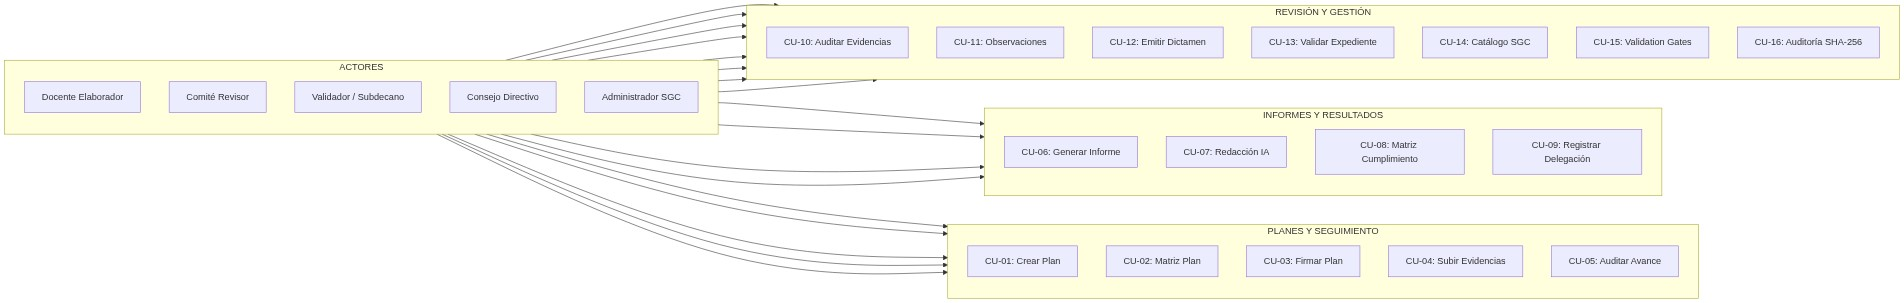
\includegraphics[width=0.88\textwidth,height=5.2cm,keepaspectratio]{images/s2_01_casos_de_uso.png}
    \caption{Diagrama General de Casos de Uso del Sistema SIGE.}
    \label{fig:s2_01_cu}
\end{figure}

El sistema estructura sus casos de uso en 4 módulos operativos principales:
\begin{enumerate}[leftmargin=1.5em, itemsep=2pt]
    \item \textbf{Módulo 1: Planificación SI UTA y Cascada al Inicio:}
    \begin{itemize}[leftmargin=1.2em]
        \item \textbf{CU-01:} Crear Plan de Trabajo en SI UTA (Ordinario).
        \item \textbf{CU-17:} Habilitar Planificación Extemporánea (Admin).
        \item \textbf{CU-02:} Gestionar Matriz de Actividades (\texttt{UTA-SGC-A-2-1-P7-T1}).
        \item \textbf{CU-03A:} Estampar Firma 1 en Cascada Inicial (Docente Responsable -- Elaborado por).
        \item \textbf{CU-03B:} Estampar Firma 2 en Cascada Inicial (Coord. Área de Conocimiento -- Revisado por).
        \item \textbf{CU-03C:} Estampar Firma 3 en Cascada Inicial (Coord. Carrera -- Aprobado por $\rightarrow$ Pasa a Ejecución).
    \end{itemize}
    \item \textbf{Módulo 2: Ejecución de la Matriz y Carga Oportuna:}
    \begin{itemize}[leftmargin=1.2em]
        \item \textbf{CU-04:} Subir Evidencia por Actividad de la Matriz Culminada en Tiempo.
        \item \textbf{CU-05:} Auditar Evidencia y \% Cumplimiento (Coord. Área).
        \item \textbf{CU-18:} Solicitar Modificación / Reprogramación de la Matriz.
        \item \textbf{CU-19:} Autorizar Modificación de la Matriz de Planificación.
    \end{itemize}
    \item \textbf{Módulo 3: Rendición de Cuentas (\texttt{UTA-SGC-A-2-1-P7-T2}):}
    \begin{itemize}[leftmargin=1.2em]
        \item \textbf{CU-06:} Generar Informe Pre-cargando la Matriz Completa Auditada.
        \item \textbf{CU-07:} Redactar Antecedentes y Conclusiones.
        \item \textbf{CU-09:} Registrar Contactos / Delegación.
        \item \textbf{CU-12:} Estampar Firma 1 en Cascada Final (Docente Responsable).
        \item \textbf{CU-13:} Estampar Firma 2 en Cascada Final (Coord. Área de Conocimiento).
        \item \textbf{CU-20:} Estampar Firma 3 en Cascada Final (Coord. Carrera $\rightarrow$ Legalización SGC).
    \end{itemize}
    \item \textbf{Módulo 4: Administración y SGC:}
    \begin{itemize}[leftmargin=1.2em]
        \item \textbf{CU-14:} Administrar Catálogo de Actividades en BD.
        \item \textbf{CU-15:} Parametrizar Calendario y Reglas de Negocio.
        \item \textbf{CU-16:} Consultar Logs de Auditoría SHA-256.
    \end{itemize}
\end{enumerate}

\section{Especificación Detallada de Casos de Uso Principales}

\subsection{CU-03A, CU-03B y CU-03C: Cascada de Firmas al Inicio (FISEI - UTA)}
\begin{itemize}[leftmargin=1.5em, itemsep=2pt]
    \item \textbf{Actores Oficiales:}
    \begin{enumerate}[leftmargin=1.2em, itemsep=1pt]
        \item \textbf{Docente Responsable:} Firma en calidad de \textit{"Elaborado por"}.
        \item \textbf{Coordinador del Área de Conocimiento:} Firma en calidad de \textit{"Revisado por"} (evalúa articulación de contenidos y APE).
        \item \textbf{Coordinador de Carrera:} Firma en calidad de \textit{"Aprobado por"} (constata articulación con el Plan de Estudios de la FISEI).
    \end{enumerate}
    \item \textbf{Precondición:} El docente ha completado el 100\% de la \textbf{Matriz de Actividades} conforme al formato oficial \texttt{UTA-SGC-A-2-1-P7-T1}.
    \item \textbf{Flujo en Cascada Inicial:}
    \begin{enumerate}[leftmargin=1.2em, itemsep=2pt]
        \item \textbf{Firma 1 (Elaborado por):} El docente revisa la Matriz de Actividades y estampa su firma electrónica (.p12 / FirmaEC). El sistema valida la matriz, bloquea el formulario al docente y promueve el Plan a \texttt{PLAN\_PENDIENTE\_FIRMA\_COORD\_AREA}.
        \item \textbf{Firma 2 (Revisado por):} El Coordinador del Área de Conocimiento accede al expediente. Verifica que la Firma 1 esté presente y válida. Si aprueba los contenidos y cronograma, estampa su firma electrónica. El Plan asciende a \texttt{PLAN\_PENDIENTE\_FIRMA\_COORD\_CARRERA}. \textit{(Si observa la matriz, rechaza a \texttt{PLAN\_OBSERVADO\_DEVUELTO} con versión V02)}.
        \item \textbf{Firma 3 (Aprobado por):} El Coordinador de Carrera verifica que existan las firmas 1 y 2. Al constatar la conformidad con el Plan de Estudios vigente de la facultad, estampa la tercera firma oficial.
        \item \textbf{Paso a Ejecución:} Al completarse la 3ra firma de la cascada inicial, el sistema cambia el estado automáticamente a \textbf{\texttt{EN\_EJECUCION}}.
    \end{enumerate}
    \item \textbf{Postcondición:} Plan aprobado con total validez legal y académica; el docente inicia formalmente la ejecución de la Matriz.
\end{itemize}

\subsection{CU-04: Subir Evidencias por Actividad de la Matriz Culminada en Tiempo}
\begin{itemize}[leftmargin=1.5em, itemsep=2pt]
    \item \textbf{Actor Principal:} Docente Responsable.
    \item \textbf{Precondición:} El Plan está en estado \texttt{EN\_EJECUCION} y se cumple la \texttt{FechaHasta} de una actividad de la \textbf{Matriz de Actividades}.
    \item \textbf{Flujo Principal:}
    \begin{enumerate}[leftmargin=1.2em, itemsep=1.5pt]
        \item El docente ingresa al panel de \textit{Seguimiento de la Matriz de Actividades} en el SI UTA.
        \item Al concluir una actividad en tiempo, selecciona la fila de la matriz y adjunta el medio de verificación en \textbf{MinIO S3}.
        \item Registra el porcentaje de cumplimiento real ($0\%$ a $100\%$).
        \item El sistema genera el hash SHA-256 inmutable de la evidencia y notifica al Coordinador del Área de Conocimiento para su validación inmediata.
    \end{enumerate}
    \item \textbf{Postcondición:} La actividad queda sustentada oportunamente sin acumular evidencias al cierre del semestre.
\end{itemize}

\subsection{CU-18: Solicitar Modificación / Reprogramación de la Matriz de Actividades}
\begin{itemize}[leftmargin=1.5em, itemsep=2pt]
    \item \textbf{Actor Principal:} Docente Responsable.
    \item \textbf{Precondición:} El Plan está en estado \texttt{EN\_EJECUCION} y se requiere reprogramar fechas \texttt{Desde}--\texttt{Hasta}, actividades de APE o recursos.
    \item \textbf{Flujo Principal:}
    \begin{enumerate}[leftmargin=1.2em, itemsep=1.5pt]
        \item El docente selecciona la opción \textit{Solicitar Modificación de la Matriz}.
        \item Ingresa la justificación técnica de la necesidad de cambio y adjunta memorando de soporte.
        \item Propone las modificaciones puntuales sobre las filas de la \textbf{Matriz de Actividades}.
        \item El Coordinador de Área y el Coordinador de Carrera evalúan la solicitud.
        \item De ser aprobada, el sistema genera la nueva versión oficial del Plan (\texttt{V02}, \texttt{V03}...) y actualiza el cronograma de ejecución de la matriz, conservando el histórico inmutable.
    \end{enumerate}
    \item \textbf{Postcondición:} Matriz de actividades reprogramada oficialmente con trazabilidad total.
\end{itemize}

\vspace{0.3cm}

% =============================================================
% FIRMAS DE RESPONSABILIDAD
% =============================================================
\section{Firmas de Responsabilidad}

\noindent
\renewcommand{\arraystretch}{1.2}
\begin{tabularx}{\textwidth}{|>{\raggedright\arraybackslash}m{2.9cm}|>{\raggedright\arraybackslash}X|>{\centering\arraybackslash}m{4.6cm}|>{\centering\arraybackslash}m{2.3cm}|}
    \hline
    \rowcolor{headerred}
    \textcolor{white}{\textbf{ACCIÓN}} & \textcolor{white}{\textbf{NOMBRE Y CARGO}} & \textcolor{white}{\textbf{FIRMA}} & \textcolor{white}{\textbf{FECHA}} \\
    \hline
    \textbf{Elaborado por:} & Heidy Villavicencio\newline \textit{Analista de Requerimientos / UI-UX} & \parbox[c]{4.4cm}{\centering\vspace{4pt}
\includegraphics[height=1.5cm,width=4.0cm,keepaspectratio]{images/firma_heidi.png}\vspace{4pt}} & 27/08/2026 \\
    \hline
    \textbf{Revisado por:} & Steeven Toala\newline \textit{Líder de Proyecto / Arquitecto Software} & \parbox[c]{4.4cm}{\centering\vspace{10pt}\textbf{\textcolor{gray!80}{\scriptsize [ PENDIENTE DE REVISIÓN ]}}\vspace{10pt}} & \textbf{\textcolor{gray!90}{Pendiente}} \\
    \hline
    \textbf{Aprobado por:} & Ing. Paulo Torres\newline \textit{Docente Tutor - Gestión Proyectos Software} & \parbox[c]{4.4cm}{\centering\vspace{10pt}\textbf{\textcolor{gray!80}{\scriptsize [ PENDIENTE DE APROBACIÓN ]}}\vspace{10pt}} & \textbf{\textcolor{gray!90}{Pendiente}} \\
    \hline
\end{tabularx}

\vspace{0.4cm}

% =============================================================
% CONTROL DE CAMBIOS
% =============================================================
\section{Control de Cambios}

\noindent
\renewcommand{\arraystretch}{1.2}
\begin{tabularx}{\textwidth}{|>{\hsize=0.45\hsize\centering\arraybackslash}X|>{\hsize=1.55\hsize\raggedright\arraybackslash}X|>{\hsize=1.2\hsize\raggedright\arraybackslash}X|>{\hsize=0.8\hsize\centering\arraybackslash}X|}
    \hline
    \rowcolor{gray!20}
    \textbf{Versión} & \textbf{Descripción del cambio} & \textbf{Responsable del cambio} & \textbf{Fecha de aprobación} \\
    \hline
    1.0 & Modelado UML general y especificación detallada de casos de uso (CU-03, CU-04, CU-18) / Pendiente de revisión & Heidy Villavicencio & \textbf{\textcolor{gray!90}{Pendiente de Revisión}} \\
    \hline
\end{tabularx}

\vspace{0.4cm}

\section{Anexos}
\subsection*{Anexo 1: Catálogo Extendido de Casos de Uso del Sistema SIGE}
Documento técnico complementario con especificaciones detalladas de los casos de uso CU-01 al CU-20 para todos los roles acreditados.

\end{document}
